\documentclass{article}

\usepackage{amsmath,amssymb}
\usepackage{tikz}
\usepackage{pgfplots}
\usepackage{xcolor}
\usepackage{colortbl}
\usepackage[left=2.1cm,right=3.1cm,bottom=3cm,footskip=0.75cm,headsep=0.5cm]{geometry}
\usepackage{enumerate}
\usepackage{enumitem}
\usepackage{marvosym}
\usepackage{tabularx}
\usepackage[amsmath,thmmarks,standard]{ntheorem}
\usepackage{mathtools}

\usepackage[utf8]{inputenc}

\renewcommand*{\arraystretch}{1.4}
\newcommand{\E}{\mathbb{E}}

\newcolumntype{L}[1]{>{\raggedright\arraybackslash}p{#1}}
\newcolumntype{R}[1]{>{\raggedleft\arraybackslash}p{#1}}
\newcolumntype{C}[1]{>{\centering\let\newline\\\arraybackslash\hspace{0pt}}m{#1}}

\DeclareMathOperator{\tr}{tr}
\DeclareMathOperator{\Var}{Var}
\DeclareMathOperator{\Cov}{Cov}
\renewcommand{\E}{\mathbb{E}}

\newtheorem{thm}{Theorem}
\newtheorem{lem}{Lemma}

\title{\textbf{Einführung in die Logistik, Übung 4}}
\author{\textsc{Henry Haustein}}
\date{}

\begin{document}
	\maketitle
	
	\section*{Aufgabe 10}
	\begin{enumerate}[label=(\alph*)]
		\item Quelle: Knoten 1, Senke: Knoten 3
		\item schwach zusammenhängend, da nicht jeder Knoten mit jedem Knoten verbunden ist
		\item Suche nach maximalen Wegen
		\begin{center}
			\begin{tabular}{c|ccccc}
				$W^0$ & 1 & 2 & 3 & 4 & 5 \\
				\hline
				1 & 1 & 1 & $\infty$ & 1 & 1 \\
				2 & $\infty$ & 2 & 2 & $\infty$ & $\infty$ \\
				3 & $\infty$ & $\infty$ & 3 & $\infty$ & $\infty$ \\
				4 & $\infty$ & $\infty$ & 4 & 4 & 4 \\
				5 & $\infty$ & 5 & $\infty$ & $\infty$ & 5
			\end{tabular}
			\begin{tabular}{c|ccccc}
				$D^0$ & 1 & 2 & 3 & 4 & 5 \\
				\hline
				1 & 0 & 5 & $-\infty$ & 3 & 10 \\
				2 & $-\infty$ & 0 & 6 & $-\infty$ & $-\infty$ \\
				3 & $-\infty$ & $-\infty$ & 0 & $-\infty$ & $-\infty$ \\
				4 & $-\infty$ & $-\infty$ & 8 & 0 & 6 \\
				5 & $-\infty$ & 8 & $-\infty$ & $-\infty$ & 0
			\end{tabular}
		\end{center}
		\begin{center}
			\begin{tabular}{c|ccccc}
				$W^2$ & 1 & 2 & 3 & 4 & 5 \\
				\hline
				1 & 1 & \cellcolor{blue!20}1 & 2 & 1 & 1 \\
				2 & \cellcolor{blue!20}$\infty$ & \cellcolor{blue!20}2 & \cellcolor{blue!20}2 & \cellcolor{blue!20}$\infty$ & \cellcolor{blue!20}$\infty$ \\
				3 & $\infty$ & \cellcolor{blue!20}$\infty$ & 3 & $\infty$ & $\infty$ \\
				4 & $\infty$ & \cellcolor{blue!20}$\infty$ & 4 & 4 & 4 \\
				5 & $\infty$ & \cellcolor{blue!20}5 & 2 & $\infty$ & 5
			\end{tabular}
			\begin{tabular}{c|ccccc}
				$D^2$ & 1 & 2 & 3 & 4 & 5 \\
				\hline
				1 & 0 & \cellcolor{blue!20}5 & 11 & 3 & 10 \\
				2 & \cellcolor{blue!20}$-\infty$ & \cellcolor{blue!20}0 & \cellcolor{blue!20}6 & \cellcolor{blue!20}$-\infty$ & \cellcolor{blue!20}$-\infty$ \\
				3 & $-\infty$ & \cellcolor{blue!20}$-\infty$ & 0 & $-\infty$ & $-\infty$ \\
				4 & $-\infty$ & \cellcolor{blue!20}$-\infty$ & 8 & 0 & 6 \\
				5 & $-\infty$ & \cellcolor{blue!20}8 & 14 & $-\infty$ & 0
			\end{tabular}
		\end{center}
		\begin{center}
			\begin{tabular}{c|ccccc}
				$W^4$ & 1 & 2 & 3 & 4 & 5 \\
				\hline
				1 & 1 & 1 & 2 & \cellcolor{blue!20}1 & 1 \\
				2 & $\infty$ & 2 & 2 & \cellcolor{blue!20}$\infty$ & $\infty$ \\
				3 & $\infty$ & $\infty$ & 3 & \cellcolor{blue!20}$\infty$ & $\infty$ \\
				4 & \cellcolor{blue!20}$\infty$ & \cellcolor{blue!20}$\infty$ & \cellcolor{blue!20}4 & \cellcolor{blue!20}4 & \cellcolor{blue!20}4 \\
				5 & $\infty$ & 5 & 2 & \cellcolor{blue!20}$\infty$ & 5
			\end{tabular}
			\begin{tabular}{c|ccccc}
				$D^4$ & 1 & 2 & 3 & 4 & 5 \\
				\hline
				1 & 0 & 5 & 11 & \cellcolor{blue!20}3 & 10 \\
				2 & $-\infty$ & 0 & 6 & \cellcolor{blue!20}$-\infty$ & $-\infty$ \\
				3 & $-\infty$ & $-\infty$ & 0 & \cellcolor{blue!20}$-\infty$ & $-\infty$ \\
				4 & \cellcolor{blue!20}$-\infty$ & \cellcolor{blue!20}$-\infty$ & \cellcolor{blue!20}8 & \cellcolor{blue!20}0 & \cellcolor{blue!20}6 \\
				5 & $-\infty$ & 8 & 14 & \cellcolor{blue!20}$-\infty$ & 0
			\end{tabular}
		\end{center}
		\begin{center}
			\begin{tabular}{c|ccccc}
				$W^5$ & 1 & 2 & 3 & 4 & 5 \\
				\hline
				1 & 1 & 5 & 5 & 1 & \cellcolor{blue!20}1 \\
				2 & $\infty$ & 2 & 2 & $\infty$ & \cellcolor{blue!20}$\infty$ \\
				3 & $\infty$ & $\infty$ & 3 & $\infty$ & \cellcolor{blue!20}$\infty$ \\
				4 & $\infty$ & 5 & 5 & 4 & \cellcolor{blue!20}4 \\
				5 & \cellcolor{blue!20}$\infty$ & \cellcolor{blue!20}5 & \cellcolor{blue!20}2 & \cellcolor{blue!20}$\infty$ & \cellcolor{blue!20}5
			\end{tabular}
			\begin{tabular}{c|ccccc}
				$D^5$ & 1 & 2 & 3 & 4 & 5 \\
				\hline
				1 & 0 & 18 & 24 & 3 & \cellcolor{blue!20}10 \\
				2 & $-\infty$ & 0 & 6 & $-\infty$ & \cellcolor{blue!20}$-\infty$ \\
				3 & $-\infty$ & $-\infty$ & 0 & $-\infty$ & \cellcolor{blue!20}$-\infty$ \\
				4 & $-\infty$ & 14 & 20 & 0 & \cellcolor{blue!20}6 \\
				5 & \cellcolor{blue!20}$-\infty$ & \cellcolor{blue!20}8 & \cellcolor{blue!20}14 & \cellcolor{blue!20}$-\infty$ & \cellcolor{blue!20}0
			\end{tabular}
		\end{center}
		Längster Weg von 1 nach 3: 1 - 5 - 2 - 3 = 24
		\item Es entsteht ein Zyklus: 2 - 4 - 5 - 2 $\Rightarrow$ Triple-Algorithmus nicht mehr anwendbar
		\item Triple-Algorithmus: Distanz von allen zu allen Knoten, Baumalgorithmen: Distanz von einem Knoten zu allen Knoten
	\end{enumerate}

	\section*{Aufgabe 11}
	\begin{enumerate}[label=(\alph*)]
		\item Graph:
		\begin{center}
			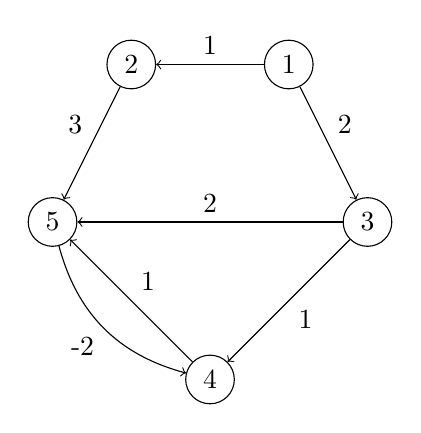
\begin{tikzpicture}
				\node[circle,draw=black, fill=white] (1) at (2,0) {1};
				\node[circle,draw=black, fill=white] (2) at (0,0) {2};
				\node[circle,draw=black, fill=white] (3) at (3,-2) {3};
				\node[circle,draw=black, fill=white] (4) at (1,-4) {4};
				\node[circle,draw=black, fill=white] (5) at (-1,-2) {5};
				
				\draw[->] (1) to node[above] {1} (2);
				\draw[->] (1) to node[above right] {2} (3);
				\draw[->] (2) to node[above left] {3} (5);
				\draw[->] (3) to node[below right] {1} (4);
				\draw[->] (3) to node[above] {2} (5);
				\draw[->] (4) to node[above right] {1} (5);
				\draw[->] (5) to[bend right=30] node[below left] {-2} (4);
			\end{tikzpicture}
		\end{center}
		\item Graph enthält negative Zyklen zwischen 4 und 5 $\Rightarrow$ Triple-Algorithmus nicht anwendbar. Zudem enthält der Graph eine negative Bewertung, damit ist der Dijkstra-Algorithmus nicht anwendbar.
	\end{enumerate}

	\section*{Aufgabe 12}
	Die Matrizen lauten
	\begin{center}
		\begin{tabular}{c|ccccc}
			$W^0$ & 1 & 2 & 3 & 4 & 5 \\
			\hline
			1 & 1 & 1 & 1 & 1 & 1 \\
			2 & $\infty$ & 2 & $\infty$ & 2 & 2 \\
			3 & $\infty$ & 3 & 3 & $\infty$ & 3 \\
			4 & $\infty$ & $\infty$ & 4 & 4 & 4 \\
			5 & $\infty$ & $\infty$ & $\infty$ & $\infty$ & 5
		\end{tabular}
		\begin{tabular}{c|ccccc}
			$D^0$ & 1 & 2 & 3 & 4 & 5 \\
			\hline
			1 & 0 & 3 & 2 & 5 & 8 \\
			2 & $\infty$ & 0 & $\infty$ & 1 & 6 \\
			3 & $\infty$ & 1 & 0 & $\infty$ & 5 \\
			4 & $\infty$ & $\infty$ & 2 & 0 & 4 \\
			5 & $\infty$ & $\infty$ & $\infty$ & $\infty$ & 0
		\end{tabular}
	\end{center}
	\begin{center}
		\begin{tabular}{c|ccccc}
			$W^2$ & 1 & 2 & 3 & 4 & 5 \\
			\hline
			1 & 1 & \cellcolor{blue!20}1 & 1 & 2 & 1 \\
			2 & \cellcolor{blue!20}$\infty$ & \cellcolor{blue!20}2 & \cellcolor{blue!20}$\infty$ & \cellcolor{blue!20}2 & \cellcolor{blue!20}2 \\
			3 & $\infty$ & \cellcolor{blue!20}3 & 3 & 2 & 3 \\
			4 & $\infty$ & \cellcolor{blue!20}$\infty$ & 4 & 4 & 4 \\
			5 & $\infty$ & \cellcolor{blue!20}$\infty$ & $\infty$ & $\infty$ & 5
		\end{tabular}
		\begin{tabular}{c|ccccc}
			$D^2$ & 1 & 2 & 3 & 4 & 5 \\
			\hline
			1 & 0 & \cellcolor{blue!20}3 & 2 & 4 & 8 \\
			2 & \cellcolor{blue!20}$\infty$ & \cellcolor{blue!20}0 & \cellcolor{blue!20}$\infty$ & \cellcolor{blue!20}1 & \cellcolor{blue!20}6 \\
			3 & $\infty$ & \cellcolor{blue!20}1 & 0 & 2 & 5 \\
			4 & $\infty$ & \cellcolor{blue!20}$\infty$ & 2 & 0 & 4 \\
			5 & $\infty$ & \cellcolor{blue!20}$\infty$ & $\infty$ & $\infty$ & 0
		\end{tabular}
	\end{center}
	\begin{center}
		\begin{tabular}{c|ccccc}
			$W^3$ & 1 & 2 & 3 & 4 & 5 \\
			\hline
			1 & 1 & 1 & \cellcolor{blue!20}1 & 2 & 3 \\
			2 & $\infty$ & 2 & \cellcolor{blue!20}$\infty$ & 2 & 2 \\
			3 & \cellcolor{blue!20}$\infty$ & \cellcolor{blue!20}3 & \cellcolor{blue!20}3 & \cellcolor{blue!20}2 & \cellcolor{blue!20}3 \\
			4 & $\infty$ & 3 & \cellcolor{blue!20}4 & 4 & 4 \\
			5 & $\infty$ & $\infty$ & \cellcolor{blue!20}$\infty$ & $\infty$ & 5
		\end{tabular}
		\begin{tabular}{c|ccccc}
			$D^3$ & 1 & 2 & 3 & 4 & 5 \\
			\hline
			1 & 0 & 3 & \cellcolor{blue!20}2 & 4 & 7 \\
			2 & $\infty$ & 0 & \cellcolor{blue!20}$\infty$ & 1 & 6 \\
			3 & \cellcolor{blue!20}$\infty$ & \cellcolor{blue!20}1 & \cellcolor{blue!20}0 & \cellcolor{blue!20}2 & \cellcolor{blue!20}5 \\
			4 & $\infty$ & 3 & \cellcolor{blue!20}2 & 0 & 4 \\
			5 & $\infty$ & $\infty$ & \cellcolor{blue!20}$\infty$ & $\infty$ & 0
		\end{tabular}
	\end{center}
	\begin{center}
		\begin{tabular}{c|ccccc}
			$W^4$ & 1 & 2 & 3 & 4 & 5 \\
			\hline
			1 & 1 & 1 & 1 & \cellcolor{blue!20}2 & 3 \\
			2 & $\infty$ & 2 & 4 & \cellcolor{blue!20}2 & 4 \\
			3 & $\infty$ & 3 & 3 & \cellcolor{blue!20}2 & 3 \\
			4 & \cellcolor{blue!20}$\infty$ & \cellcolor{blue!20}3 & \cellcolor{blue!20}4 & \cellcolor{blue!20}4 & \cellcolor{blue!20}4 \\
			5 & $\infty$ & $\infty$ & $\infty$ & \cellcolor{blue!20}$\infty$ & 5
		\end{tabular}
		\begin{tabular}{c|ccccc}
			$D^4$ & 1 & 2 & 3 & 4 & 5 \\
			\hline
			1 & 0 & 3 & 2 & \cellcolor{blue!20}4 & 7 \\
			2 & $\infty$ & 0 & 3 & \cellcolor{blue!20}1 & 5 \\
			3 & $\infty$ & 1 & 0 & \cellcolor{blue!20}2 & 5 \\
			4 & \cellcolor{blue!20}$\infty$ & \cellcolor{blue!20}3 & \cellcolor{blue!20}2 & \cellcolor{blue!20}0 & \cellcolor{blue!20}4 \\
			5 & $\infty$ & $\infty$ & $\infty$ & \cellcolor{blue!20}$\infty$ & 0
		\end{tabular}
	\end{center}
	\begin{center}
		\begin{tabular}{c|ccccc}
			$W^5$ & 1 & 2 & 3 & 4 & 5 \\
			\hline
			1 & 1 & 1 & 1 & 2 & \cellcolor{blue!20}3 \\
			2 & $\infty$ & 2 & 4 & 2 & \cellcolor{blue!20}4 \\
			3 & $\infty$ & 3 & 3 & 2 & \cellcolor{blue!20}3 \\
			4 & $\infty$ & 3 & 4 & 4 & \cellcolor{blue!20}4 \\
			5 & \cellcolor{blue!20}$\infty$ & \cellcolor{blue!20}$\infty$ & \cellcolor{blue!20}$\infty$ & \cellcolor{blue!20}$\infty$ & \cellcolor{blue!20}5
		\end{tabular}
		\begin{tabular}{c|ccccc}
			$D^5$ & 1 & 2 & 3 & 4 & 5 \\
			\hline
			1 & 0 & 3 & 2 & 4 & \cellcolor{blue!20}7 \\
			2 & $\infty$ & 0 & 3 & 1 & \cellcolor{blue!20}5 \\
			3 & $\infty$ & 1 & 0 & 2 & \cellcolor{blue!20}5 \\
			4 & $\infty$ & 3 & 2 & 0 & \cellcolor{blue!20}4 \\
			5 & \cellcolor{blue!20}$\infty$ & \cellcolor{blue!20}$\infty$ & \cellcolor{blue!20}$\infty$ & \cellcolor{blue!20}$\infty$ & \cellcolor{blue!20}0
		\end{tabular}
	\end{center}
	Kürzester Weg von 1 nach 3: 1 - 3 - 5 = 7

	\section*{Aufgabe 13}
	\begin{enumerate}[label=(\alph*)]
		\item Es gibt 6 Knoten, damit ist $C_1$ nicht möglich. Auch $C_2$ ist nicht möglich, da $(2,6)\in\vec{E}$, aber $C_2(2,6)=\infty$. Nur $C_3$ ist möglich.
		\item Es gibt negative Zyklen bei $C_1$ (2 $\to$ 3, 3 $\to$ 2) und bei $C_3$ (2 $\to$ 4, 4 $\to$ 2). Nur $C_2$ ist möglich.
		\begin{center}
			\begin{tabular}{c|cccc}
				$W^0$ & 1 & 2 & 3 & 4 \\
				\hline
				1 & 1 & 1 & 1 & 1 \\
				2 & $\infty$ & 2 & 2 & 2 \\
				3 & 3 & $\infty$ & 3 & $\infty$ \\
				4 & 4 & $\infty$ & 4 & 4
			\end{tabular}
			\begin{tabular}{c|cccc}
				$D^0$ & 1 & 2 & 3 & 4 \\
				\hline
				1 & 0 & -1 & 3 & 4 \\
				2 & $\infty$ & 0 & 2 & 1 \\
				3 & 5 & $\infty$ & 0 & $\infty$ \\
				4 & 3 & $\infty$ & 2 & 0
			\end{tabular}
		\end{center}
		\begin{center}
			\begin{tabular}{c|cccc}
				$W^1$ & 1 & 2 & 3 & 4 \\
				\hline
				1 & \cellcolor{blue!20}1 & \cellcolor{blue!20}1 & \cellcolor{blue!20}1 & \cellcolor{blue!20}1 \\
				2 & \cellcolor{blue!20}$\infty$ & 2 & 2 & 2 \\
				3 & \cellcolor{blue!20}3 & 1 & 3 & 1 \\
				4 & \cellcolor{blue!20}4 & 1 & 4 & 4
			\end{tabular}
			\begin{tabular}{c|cccc}
				$D^1$ & 1 & 2 & 3 & 4 \\
				\hline
				1 & \cellcolor{blue!20}0 & \cellcolor{blue!20}-1 & \cellcolor{blue!20}3 & \cellcolor{blue!20}4 \\
				2 & \cellcolor{blue!20}$\infty$ & 0 & 2 & 1 \\
				3 & \cellcolor{blue!20}5 & 4 & 0 & 9 \\
				4 & \cellcolor{blue!20}3 & 2 & 2 & 0
			\end{tabular}
		\end{center}
		\begin{center}
			\begin{tabular}{c|cccc}
				$W^2$ & 1 & 2 & 3 & 4 \\
				\hline
				1 & 1 & \cellcolor{blue!20}1 & 2 & 2 \\
				2 & \cellcolor{blue!20}$\infty$ & \cellcolor{blue!20}2 & \cellcolor{blue!20}2 & \cellcolor{blue!20}2 \\
				3 & 3 & \cellcolor{blue!20}1 & 3 & 2 \\
				4 & 4 & \cellcolor{blue!20}1 & 4 & 4
			\end{tabular}
			\begin{tabular}{c|cccc}
				$D^2$ & 1 & 2 & 3 & 4 \\
				\hline
				1 & 0 & \cellcolor{blue!20}-1 & 1 & 0 \\
				2 & \cellcolor{blue!20}$\infty$ & \cellcolor{blue!20}0 & \cellcolor{blue!20}2 & \cellcolor{blue!20}1 \\
				3 & 5 & \cellcolor{blue!20}4 & 0 & 5 \\
				4 & 3 & \cellcolor{blue!20}2 & 2 & 0
			\end{tabular}
		\end{center}
		\begin{center}
			\begin{tabular}{c|cccc}
				$W^3$ & 1 & 2 & 3 & 4 \\
				\hline
				1 & 1 & 1 & \cellcolor{blue!20}2 & 2 \\
				2 & 3 & 2 & \cellcolor{blue!20}2 & 2 \\
				3 & \cellcolor{blue!20}3 & \cellcolor{blue!20}1 & \cellcolor{blue!20}3 & \cellcolor{blue!20}2 \\
				4 & 4 & 1 & \cellcolor{blue!20}4 & 4
			\end{tabular}
			\begin{tabular}{c|cccc}
				$D^3$ & 1 & 2 & 3 & 4 \\
				\hline
				1 & 0 & -1 & \cellcolor{blue!20}1 & 0 \\
				2 & 7 & 0 & \cellcolor{blue!20}2 & 1 \\
				3 & \cellcolor{blue!20}5 & \cellcolor{blue!20}4 & \cellcolor{blue!20}0 & \cellcolor{blue!20}5 \\
				4 & 3 & 2 & \cellcolor{blue!20}2 & 0
			\end{tabular}
		\end{center}
		\begin{center}
			\begin{tabular}{c|cccc}
				$W^4$ & 1 & 2 & 3 & 4 \\
				\hline
				1 & 1 & 1 & 2 & \cellcolor{blue!20}2 \\
				2 & 4 & 2 & 2 & \cellcolor{blue!20}2 \\
				3 & 3 & 1 & 3 & \cellcolor{blue!20}2 \\
				4 & \cellcolor{blue!20}4 & \cellcolor{blue!20}1 & \cellcolor{blue!20}4 & \cellcolor{blue!20}4
			\end{tabular}
			\begin{tabular}{c|cccc}
				$D^4$ & 1 & 2 & 3 & 4 \\
				\hline
				1 & 0 & -1 & 1 & \cellcolor{blue!20}0 \\
				2 & 4 & 0 & 2 & \cellcolor{blue!20}1 \\
				3 & 5 & 4 & 0 & \cellcolor{blue!20}5 \\
				4 & \cellcolor{blue!20}3 & \cellcolor{blue!20}2 & \cellcolor{blue!20}2 & \cellcolor{blue!20}0
			\end{tabular}
		\end{center}
	\end{enumerate}

	\section*{Aufgabe 14}
	Graph $G$: offensichtlich kreisfrei
	\begin{center}
		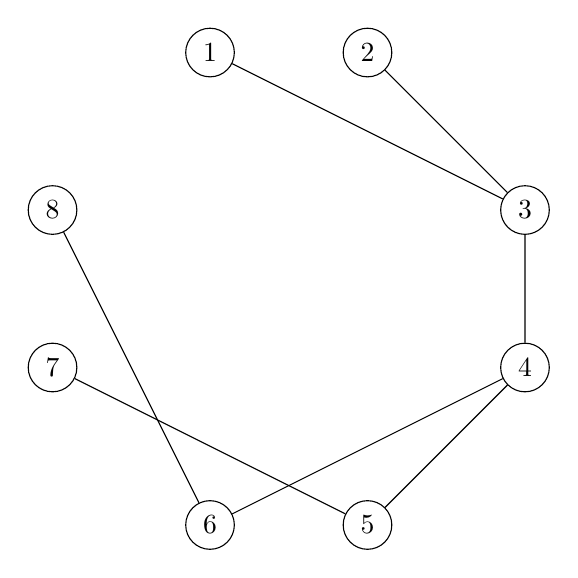
\begin{tikzpicture}
			\node[circle,draw=black, fill=white] (1) at (0,0) {1};
			\node[circle,draw=black, fill=white] (2) at (2,0) {2};
			\node[circle,draw=black, fill=white] (3) at (4,-2) {3};
			\node[circle,draw=black, fill=white] (4) at (4,-4) {4};
			\node[circle,draw=black, fill=white] (5) at (2,-6) {5};
			\node[circle,draw=black, fill=white] (6) at (0,-6) {6};
			\node[circle,draw=black, fill=white] (7) at (-2,-4) {7};
			\node[circle,draw=black, fill=white] (8) at (-2,-2) {8};
			
			\draw (1) -- (3) -- (4) -- (5) -- (7);
			\draw (2) -- (3);
			\draw (4) -- (6) -- (8);
		\end{tikzpicture}
	\end{center}
	Graph $G'$: enthält Kreis 1 - 2 - 4 - 1
	\begin{center}
		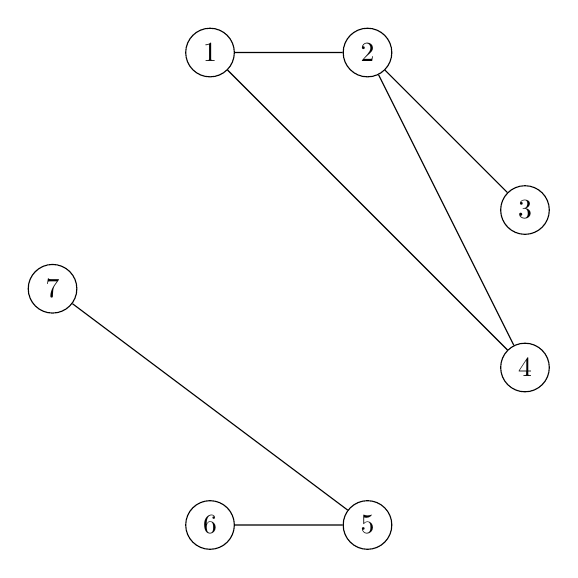
\begin{tikzpicture}
			\node[circle,draw=black, fill=white] (1) at (0,0) {1};
			\node[circle,draw=black, fill=white] (2) at (2,0) {2};
			\node[circle,draw=black, fill=white] (3) at (4,-2) {3};
			\node[circle,draw=black, fill=white] (4) at (4,-4) {4};
			\node[circle,draw=black, fill=white] (5) at (2,-6) {5};
			\node[circle,draw=black, fill=white] (6) at (0,-6) {6};
			\node[circle,draw=black, fill=white] (7) at (-2,-3) {7};
			
			\draw (1) -- (2) -- (3);
			\draw (2) -- (4) -- (1);
			\draw (6) -- (5) -- (7);
		\end{tikzpicture}
	\end{center}
	
\end{document}